%Author: Erik Belko - xbelko02

\documentclass[10pt, hyperref={unicode}, xcolor=pdflatex]{beamer}
\usepackage{newcent}
\usepackage[utf8]{inputenc}
\usepackage[slovak]{babel}
\usepackage{hyperref}
\usepackage{fancyvrb}
\usetheme{FIT}

%%%%%%%%%%%%%%%%%%%%%%%%%%%%%%%%%%%%%%%%%%%%%%%%%%%%%%%%%%%%%%%%%%
\title{Implementácia prekladača imperatívneho jazyka
IFJ20 - Tím 98}

\author{\textbf{Harvan Mário} \and Martiček Juraj \\ Belko Erik
\and Šlesár Michal}

\institute{Brno University of Technology, Faculty of Information
Technology\\
Bo\v{z}et\v{e}chova 1/2. 612 66 Brno - Kr\'alovo Pole\\}

\date{\today}

%%%%%%%%%%%%%%%%%%%%%%%%%%%%%%%%%%%%%%%%%%%%%%%%%%%%%%%%%%%%%%%%%%
\begin{document}

\frame[plain]{\titlepage}

\begin{frame}\frametitle{Prekladač}
    \begin{figure}[h]
        \scalebox{0.25}{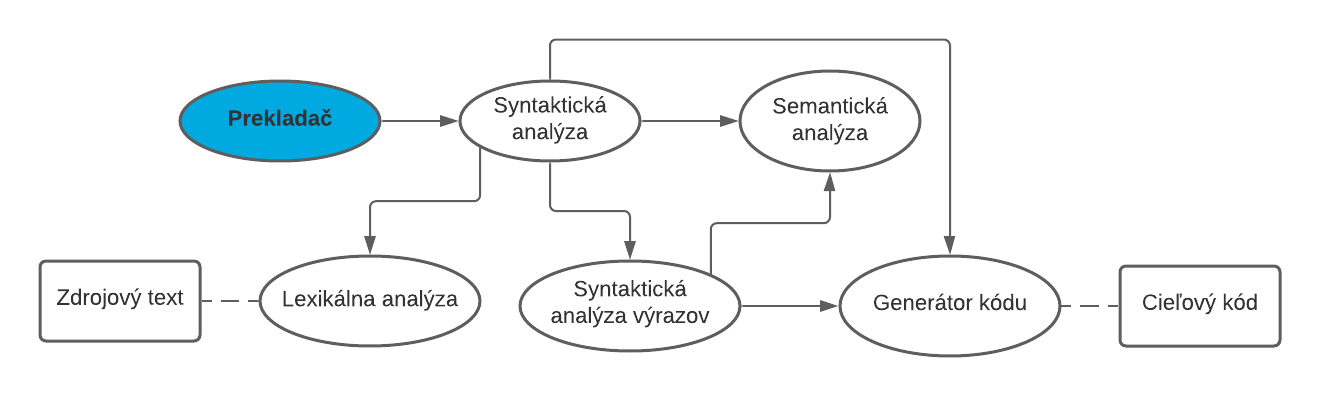
\includegraphics{img/Diagram6.png}}
    \end{figure}
    \begin{itemize}
        \item Uchovávanie užitočných dát pre syntaktickú analýzu
        \item Spúšťanie syntaktickej analýzy
    \end{itemize}
\end{frame}

\begin{frame}\frametitle{Syntaktická analýza}
    \begin{figure}[h]
        \scalebox{0.25}{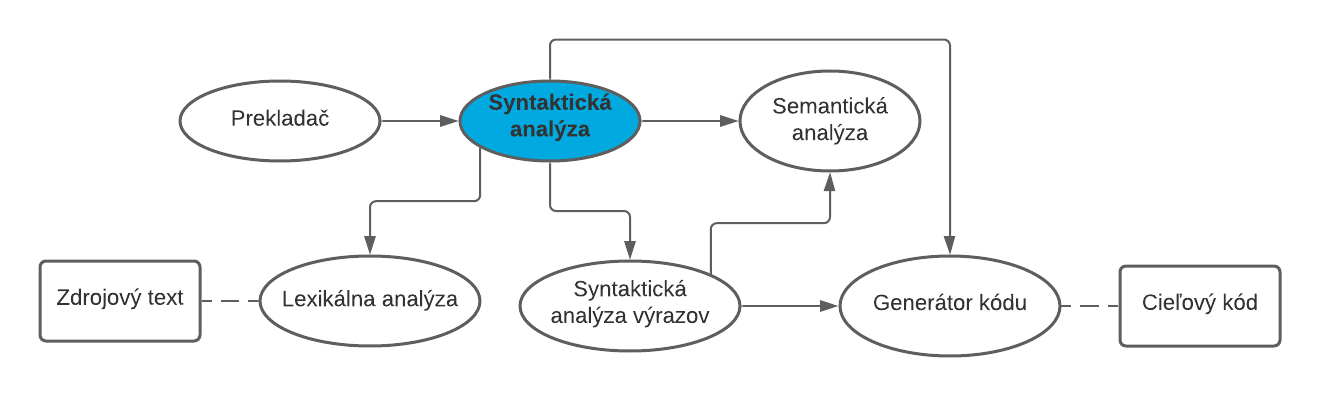
\includegraphics{img/Diagram1.png}}
    \end{figure}
    \begin{itemize}
        \item Kontrola postupnosti tokenov podla syntaxe jazyka \emph{IFJ20}
        \item \emph{1. prechod:} Spracovanie hlavičiek funkcií a~ich vloženie do~tabuľky symbolov
        \item \emph{2 prechod:} Rekurzívny zostup podľa pravidiel LL-gramatiky
    \end{itemize}
\end{frame}

\begin{frame}\frametitle{Sémantická analýza}
    \begin{figure}[h]
        \scalebox{0.25}{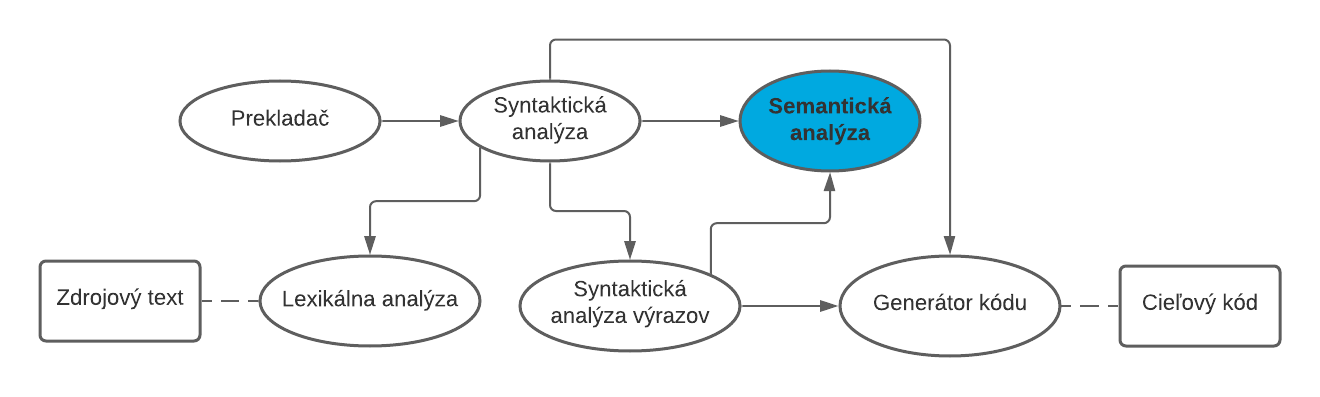
\includegraphics{img/Diagram2.png}}
    \end{figure}
    \begin{itemize}
        \item Kontrola deklarácie premenných a~funkcií
        \item Overenie rozsahu platnosti premenných
    \end{itemize}
\end{frame}

\begin{frame}\frametitle{Lexikálna analýza}
    \begin{figure}[h]
        \scalebox{0.25}{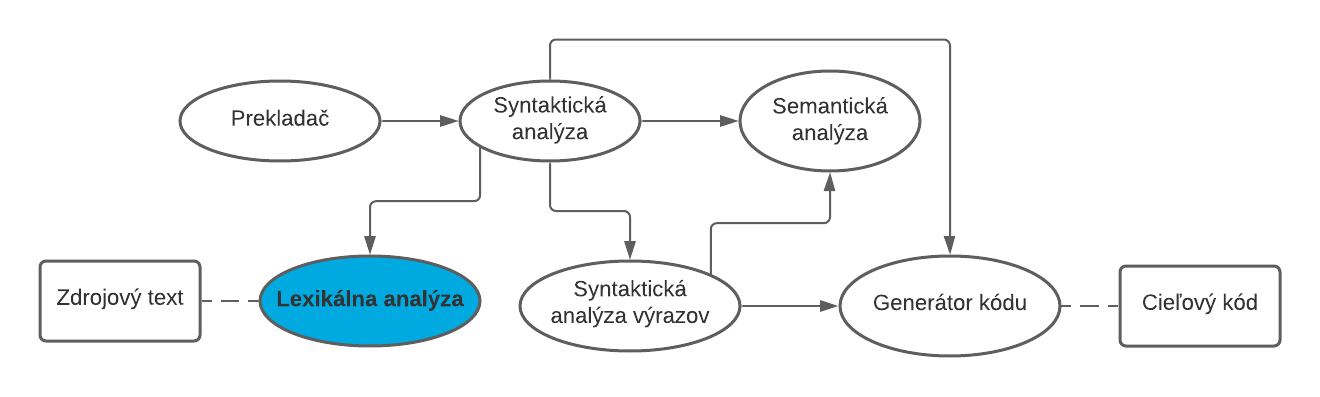
\includegraphics{img/Diagram3.png}}
    \end{figure}
    \begin{itemize}
        \item Načítavanie zdrojového kódu a~spracovanie \emph{tokenov}
        \item Implementácia na~základe \emph{konečného automatu}
    \end{itemize}
\end{frame}

\begin{frame}\frametitle{Syntaktická analýza výrazov}
    \begin{figure}[h]
        \scalebox{0.25}{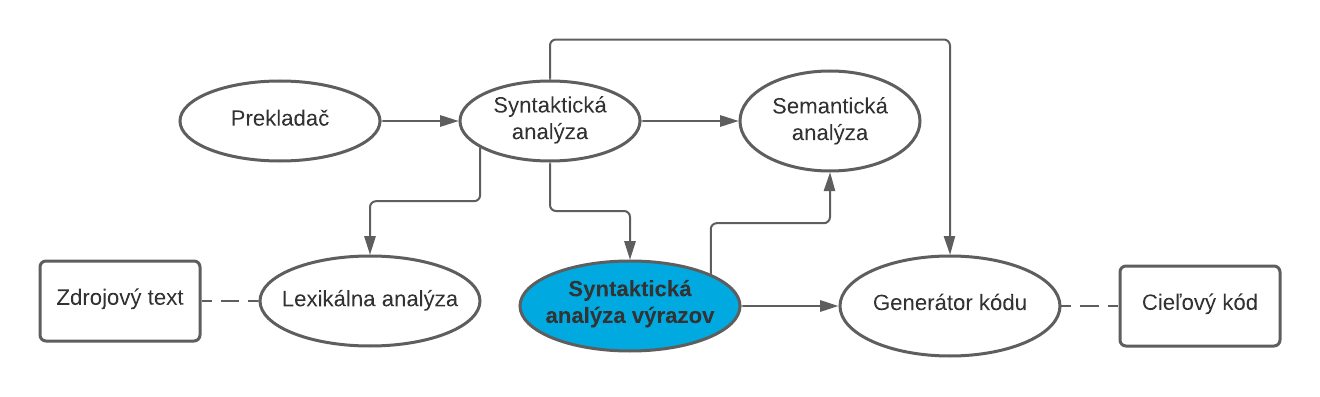
\includegraphics{img/Diagram4.png}}
    \end{figure}
    \begin{itemize}
        \item Implementácia pomocou precedenčnej analýzy
        \item Kontrola správnosti zadaných výrazov
        \item Sémantická kontrola typov operandov
    \end{itemize}
\end{frame}

\begin{frame}\frametitle{Generátor kódu}
    \begin{figure}[h]
        \scalebox{0.25}{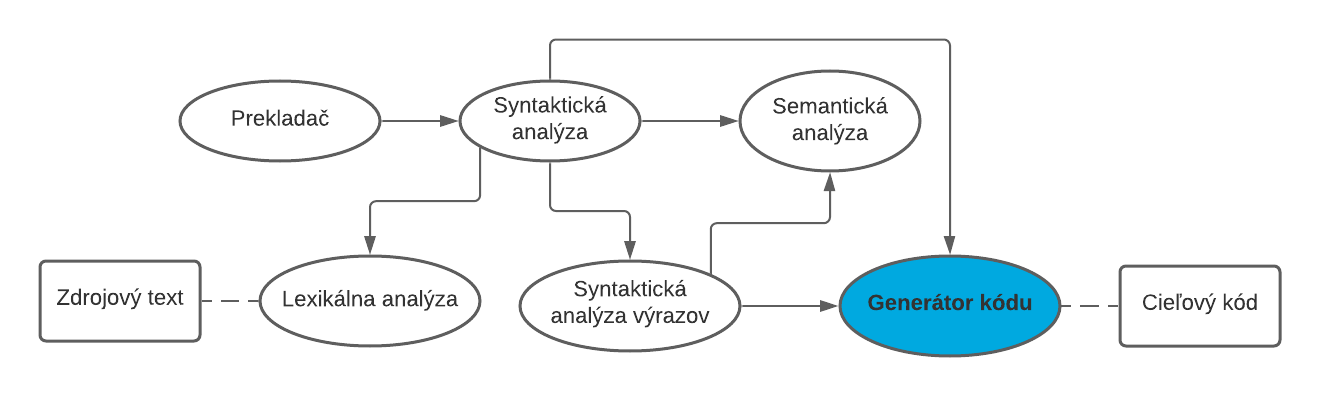
\includegraphics{img/Diagram5.png}}
    \end{figure}
    \begin{itemize}
        \item Hlavička kódu
        \item Cykly a podmienky
        \item Volanie a deklarácia funkcií
        \item Pridávane prefixov
        \item Koniec programu a error handling
    \end{itemize}
\end{frame}

\begin{frame}{Tímová práca}
    \begin{itemize}
        \item Metodika vývoja \emph{Scrum} s týždňovými šprintami
        \item \emph{GitLab} a~\emph{Discord}
        \item Pravidelná tímová komunikácia
    \end{itemize}
\end{frame}

\begin{frame}{Záver}
    Ciele a šprinty boli splnené podľa našich predstáv. \\ V tímovej spolupráci neboli žiadne problémy. \\ Vďaka projektu sme nadobudli cenné skusenosti.
\end{frame}

\begin{frame}\frametitle{Použitá literatúra}
    \begin{itemize}
        \item Prednášky a prezentácie predmetu \emph{IFJ}
        \item Prednášky a prezentácie predmetu \emph{IAL}
    \end{itemize}
\end{frame}

\bluepage{Ďakujeme za pozornosť !}

\end{document}
